\documentclass[fleqn]{article}
\oddsidemargin 0.0in
\textwidth 6.0in
\thispagestyle{empty}
\usepackage{import}
\usepackage{amsmath}
\usepackage{graphicx}
\usepackage{flexisym}
\usepackage{calligra}
\usepackage{amssymb}
\usepackage{bigints} 
\usepackage[english]{babel}
\usepackage[utf8x]{inputenc}
\usepackage{float}
\usepackage[colorinlistoftodos]{todonotes}


\DeclareMathAlphabet{\mathcalligra}{T1}{calligra}{m}{n}
\DeclareFontShape{T1}{calligra}{m}{n}{<->s*[2.2]callig15}{}
\newcommand{\scriptr}{\mathcalligra{r}\,}
\newcommand{\boldscriptr}{\pmb{\mathcalligra{r}}\,}

\definecolor{hwColor}{HTML}{442020}

\begin{document}

  \begin{titlepage}

    \newcommand{\HRule}{\rule{\linewidth}{0.5mm}}

    \center

    \begin{center}
      
\includegraphics[height=11cm, width=11cm]{asu.png}
    \end{center}

    \vline

    \textsc{\LARGE Statistical/Thermal Physics}\\[1.5cm]

    \HRule \\[0.5cm]
    { \huge \bfseries Exam 2}\\[0.4cm] 
    \HRule \\[1.0cm]

    \textbf{Behnam Amiri}

    \bigbreak

    \textbf{Prof: Michael Treacy}

    \bigbreak

    \textbf{{\large \today}\\[2cm]}

    \vfill

  \end{titlepage}

  By signing my name, I am promising that I did this quiz on my own without any outside help.

  \vspace{0.5cm}

  Name: \textbf{Behnam Amiri}

  \vspace{1cm}

  \begin{enumerate}
    \item Suppose you flip $20$ fair coins.
    \begin{enumerate}
      \item (5 points) How many possible outcomes (microstates) are there?


      \item (5 points) How many ways are there of getting exactly 10 heads and 10 tails?


      \item (5 points) What is the probability (between 0 and 1) of getting exactly 10 heads and 10
      tails?

    \end{enumerate}


    \item (15 points) A container with $0.2$ moles of $O_2$ and a container with $0.8$ moles of $N_2$ are connected
    by a closed valve. Both containers are initially at STP. The valve is opened. After some time,
    the gases are thoroughly mixed, quasistatically, by diffusion. What is the final entropy of mixing
    in $J/K$?


    \item A 1-liter container, A, holding 0$.1$ mole of air at $20^{\circ} C$ is attached to a second 1-liter container,
    B, holding an additional $0.1$ mole of air at $100^{\circ} C$. The whole A-B assembly is insulated. The
    valve separating the containers is opened and the gases are allowed to equilibrate quasistatically.
    \begin{enumerate}
      \item (5 points) What is the equilibrium temperature (in ${}^\circ C$)?

      \item (5 points) What is the equilibrium pressure (in Pa)?


      \item (5 points) The equilibrated gas in B is now pushed by a piston quasistatically into A until chamber B
      is empty. The volume of container A remains constant. What is the final temperature (in ${}^\circ C$)?


      \item (5 points) What is the final pressure (in Pa)?


      \item (10 points) What is the overall change in entropy, ∆S, of the AB system (in J/K, from the
      start of the problem to the end)?
    \end{enumerate}

    \pagebreak
    
    \item The plot shows the measured molar specific heat, $C_p$, of methane gas, $CH_4$, at constant pressure.
    \begin{center}
      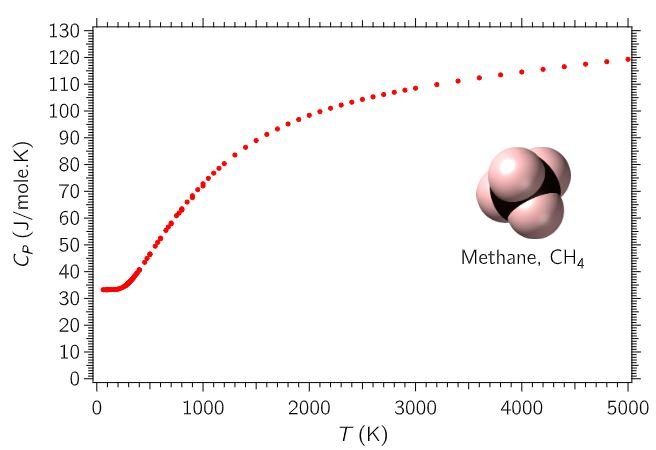
\includegraphics[height=9cm, width=13cm]{question4.JPG}
    \end{center}
    \begin{enumerate}
      \item (5 points) How many translational degrees of freedom does methane have?

      \item (5 points) What is the maximum number of rotational degrees of freedom that methane can
      have?

      \item (5 points) How many vibrational eigenmodes are there in a molecule of methane?


      \item (5 points) How many vibrational quadratic-energy degrees of freedom can methane have?


      \item (5 points) What is the maximum total number of quadratic-energy degrees of freedom, $f$,
      for methane?


      \item (5 points) If all $f$ modes were fully activated, what would be the value of the specific heat
      at constant volume, $C_v$, for methane (in $J/mole.K$)?


      \item (5 points) If all $f$ modes were fully activated, what would be the value of the specific heat
      at constant pressure, $C_p$, for methane (in $J/mole.K$)?


      \item (5 points) By examining the low-temperature end of the graph, estimate how many energy
      degrees of freedom, $f$, are active at $150 ~ K$? (Methane is a liquid below $112 ~ K$).


      \item (5 points) What do you think is happening to the methane above about $3000 ~ K$?
      \begin{enumerate}
        \item Translational modes are becoming active.

        \item Rotational modes are starting to become active.

        \item Vibrational modes are starting to become active.

        \item The equipartition theorem breaks down.

        \item The methane molecule is starting to break down.

      \end{enumerate}

    \end{enumerate}


    \item (15 points) Use the tables at the back of the Schroeder textbook to determine the chemical
    potential of methane molecules in the pure gaseous state at $298 ~ K$ and $1$ bar pressure. Give
    your answer in $eV$.



    \item The figure shows a $PV$ diagram for a cyclic process using a diatomic gas as the medium. At
    point A, the gas is at $300 ~ K$. The arrows indicate the direction of the process.
    \begin{center}
      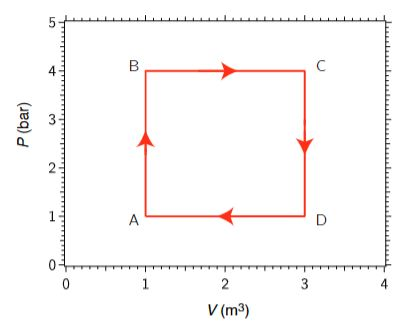
\includegraphics[height=6cm, width=9cm]{question6.JPG}
    \end{center}
    \begin{enumerate}
      \item (5 points) How many moles of gas are there?

      \item (5 points) What is the change in energy, $U$, of the gas after $N$ complete cycles (in joules)?
  
      \item (5 points) What is the work done by the gas after each cycle (in joules)?
  
      \item (5 points) What is the entropy change of the gas after each cycle (in $J/K$)?
  
      \item (5 points) If this were a heat engine, what would be the maximum efficiency of the process?
      (Give your answer as a percentage). You may assume that $c_v$ and $c_p$ remain constant over
      the cycle.
  
      \item (5 points) What would be the maximum efficiency of the process if this were a Carnot cycle
      operating between the two extreme temperatures (give your answer as a percentage)?


    \end{enumerate}


    \item A liquid-methanol ($CH_3 OH$) fuel cell uses the spontaneous redox reaction
    $$
      CH_3 OH+\dfrac{3}{2} O_2 \longrightarrow 2H_2 O+CO_2
    $$
    to generate electrical power. Some relevant thermodynamic data for this reaction (per mole, at
    2$98 ~ K$ and $1$ bar) are reproduced here from the Schroeder textbook (pp. 404-405), and from
    \emph{Lange's Handbook of Chemistry}:
    \begin{center}
      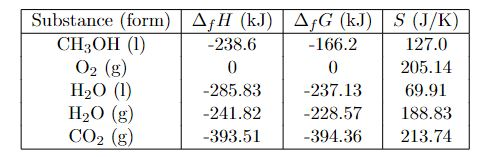
\includegraphics[height=4cm, width=9cm]{question7.JPG}
    \end{center}
    \begin{enumerate}
      \item (5 points) Use the information provided to determine the value of $\Delta H$ for this reaction, for
      one mole of methanol (in kJ). Assume that the reaction takes place at $298 ~ K$ and $1$ bar.

      \item (5 points) Use the information provided to determine the value of $\Delta G$ for this reaction, for
      one mole of methanol (in $kJ$). Assume that the reaction takes place at $298 ~ K$ and $1$ bar.


      \item (10 points) Assuming ideal performance, how much electrical work can you get out of the
      cell for each mole of methanol fuel (in $kJ$)?


      \item (10 points) How much waste heat (in kJ) is produced for each mole of methanol fuel?


      \item (10 points) Determine the voltage (in volts) of the cell if the steps of this reaction are:
      $$
        \text{Reduction at the (-) electrode :} ~~~~ CH_3 OH+H_2 O \longrightarrow CO_2+6H^++6e^-
      $$
      $$
        \text{Oxidation at the (+) electrode :} ~~~~ \dfrac{3}{2} O_2+6H^+ +6H_- \longrightarrow 3H_2 O 
      $$

    \end{enumerate}

    \item Calcium carbonate, $CaCO_3$, has two common crystalline forms, calcite and aragonite. Thermodynamic 
    data can be found at the back of the Schroeder textbook.
    \begin{enumerate}
      \item (5 points) Which is stable at the earth's surface, calcite or aragonite?

      \item (15 points) Calculate the pressure (in kbar) at which the other phase should become stable
      at room temperature.

    \end{enumerate}

    \item (20 points) A saline solution has $15 ~ g$ of $NaCl$ dissolved in $1 ~ kg$ of pure water at $300 ~ K$. Estimate
    the osmotic pressure (in bar) between the saltwater and pure water.


    \item Each atom, in a chunk of the fictitious element "metallium", contributes one conduction electron. 
    The density of metallium is $10000 ~ kg/m^3$ and its atomic weight is $100$. Determine, for
    this fictional metallium:
    \begin{enumerate}
      \item (5 points) The Fermi energy (in eV);

      \item (5 points) The Fermi temperature (in kelvin);

      \item (5 points) The degeneracy pressure (in gigapascal);

      \item (5 points) The contribution of the degeneracy pressure to the bulk modulus (in gigapascal).
      
    \end{enumerate}

  \end{enumerate}

\end{document}
